%!TEX root = ../Main.tex

\chapter{Exercise 7}

In this exercise, a custom IP called "advios" is created using SystemC. Then a test-bench is written that verifies the functionality of the IP. Using the tool "vivado HLS", the C-code is synthesized into VHDL-code. Using the aforementioned test-bench, the VHDL-code is verified to have the same funcitonlaity as the C-code.
After synthesizing the IP, a project is created, in which the IP is used in an application, and the functionality is tested through visual inspection.

\begin{figure}[b]
	\centering
	{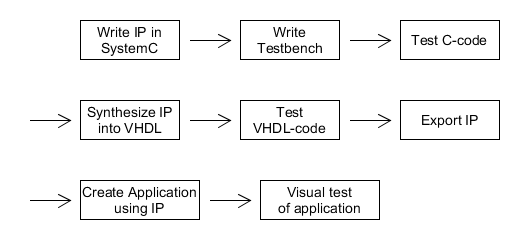
\includegraphics[scale=0.5]{Images/2_7_procedure.png}}\\[0.5cm]
	\large \date\\[0.5cm]
	\copyright \sffamily  \ \ \the\year \ - All Rights Reserved
\end{figure}